%
We firstly present three examples in detail, illustrating the $\THESYSTEM$ algorithm procedures.
The first example contains nested loop and nested.
The second examples is an data analysis algorithm used for data-base attack in real-world.
The last example example is a path-sensitive algorithm, where the $\THESYSTEM$ analysis result is over-approximated. 
Then we show our implementation results on these three examples, and few more examples without detail of the  algorithm procedures.
%
\subsection{Examples}
%
\begin{example}[Multiple Round Algorithm]
%
The two round strategy works well in our framework, we explore further to look at an advanced adaptive data analysis algorithm - multiple round algorithm.
%
%
\end{example}
%   We have seen the two round algorithm in Section~\ref{subsec:loop-syntax}. We show the multiple-round algorithm, which is an advanced algorithm.
%  \\
%
% The multiple rounds algorithm starts from an initialized empty tracking list $I$, two scores called Nscore $ns=0$ and Cscore $cs=0$, initialzied to $0$. It goes $k$ rounds and at every round, the two scores $ns$ and $cs$ are updated by the result $a$ of a query $q(f(I))$. The function $f( I)$ specifies a complex linear query using the updated tracking list $I$. The tracking list $I$ is updated by the two scores via a function $update(I,ns,cs)$ at every round. This update function mainly compares $ns$ and $cs$, when $ns \geq cs$, certain elements are added to the tracking list $I$. An implementation of the algorithm is presented in Figure~\ref{fig:multi_code}(a), in which the round number $k$ are set to $3$, and we use $update\_cscore(a)$ and $update\_nscore(a)$ to simplify the complex update on Cscore and Nscore respectively, for the sake of simplicity.
The multiple round algorithm starts from an initialized empty tracking list $I$, a score called Nscore $ns=0$ , another score Cscore $cs=0$.
There is a hidden database $D$ as well.
% a score called Nscore $ns=0$ , another score Cscore $cs=0$. There is a hidden database $X$ as well.
% It goes $k$ rounds and every round, the two scores $ns$ and $cs$ are updated by a query result. 
% Then the list $I$ is updated by the two scores for every round. After the $r$ rounds, the algorithm returns the columns of the hidden database $X$ not specified in the tracking list $I$, which is $X\setminus I$. 
It goes $k$ rounds and every round, the two scores $ns$ and $cs$ are updated by a query result. 
Then the tracking list is updated by the two scores for every round.  
% Then the list $I$ is updated by the two scores for every round. 
After the $r$ rounds, the algorithm returns the columns of the hidden database $D$ not specified in the tracking list $I$, which is $D \setminus I$. 
\\
The algorithm is written in the {\tt Query While} language as $\kw{multipleRounds(k, c)} $ taking two parameters $k$ and $c$ for 
number of iterations and the distribution sampling primitive $c$.
It starts from an initialized empty tracking list $I$ as well,
% a score called Nscore $ns=0$ , another score Cscore $cs=0$. There is a hidden database $X$ as well.
% It goes $k$ rounds and every round, the two scores $ns$ and $cs$ are updated by a query result. 
% Then the list $I$ is updated by the two scores for every round. After the $r$ rounds, the algorithm returns the columns of the hidden database $X$ not specified in the tracking list $I$, which is $X\setminus I$. 
\jl{
It goes $k$ rounds and every round, construct the query $\query(\chi[I])$
and obtain the query result $a$.
Then, the tracking list $I$ is updated by a query result. 
% Then the list $I$ is updated by the two scores for every round. 
After the $r$ rounds, the algorithm returns the columns of the hidden database $D$ not specified in the tracking list $I$.
The $\mathrel{\mathsf{update}} ( {I}, (a, p))$ function takes $I, a, p$ as input and compute the updated results for $I$.
$\mathsf{update}$ function is used here to simplify the complex update computation of Nscore, Cscore and the tracking list $I$.
It will not change our analysis because these functions provides enough information through their arguments.%
}
% It uses a loop for the $k$ rounds computation and. We use functions $update\_nscore(p,a)$,$update\_cscore(p,a)$,$update(I,ns,cs)$ to simplify the complex update computation of Nscore, Cscore and the tracking list $I$. It will not change our analysis because these functions provides enough information through their arguments.
% As described in the two round algorithm, the multi-round algorithm has a loop as well.
% compare to two round algorithm

% and the tracking list $I$. It will not change our analysis because these functions provides enough information through their arguments.
% As described in the two round algorithm, the multi-round algorithm has a loop as well.
% compare to two round algorithm
\jl{One complexity of the multiple rounds algorithm 
in comparison with the two round algorithm, the query asked in each iteration is not independent  in the multiple round one any more. 
The query in one iteration $j$ now depends on the tracking list $I$ from its previous iteration $j-1$, which is updated by the query result at the same iteration $j-1$. We can easily see the connection between queries from different iterations,  which means these queries are adaptively chosen according to our Theorem~\ref{thm:gaussiannoise2}.
}
% in comparison with the two rounds one, is that the query asked in each iteration is not independent(non-adaptive) anymore.
% For example, the query $q^{j}$ at iteration $j$ now may depend on the tracking list $I$, which comes from the previous iteration $j-1$. Additionally, this list $I$ at iteration $j-1$ is updated by the query result $q^{j-1}$ at the same iteration. Intuitively, we can see the connection between queries from different iterations, which means these queries are adaptively chosen according to our Theorem~\ref{thm:gaussiannoise2}.

% the result of the query from previous iteration,
% so that the query ask at the $j^{th}$ iteration is
% $q(p, I)$.
%
% In $MR$, the tracking list $I$ is initialized to an empty list. It appears inside the function of query $q(f(p,I))$ and updated in each iteration. 
% by the result of query in that iteration. It uses an update function $\eupdt$. 
% The input of this function is $a, p$, where $a$ is the result of the query in current iteration.
% \\
% By assuming a specific database $D = [[1, 1], [0, 0], [1, 1], [1, 1]]$,
\todo{The adaptivity through dependency graph}
\jl{
We first show its query-based dependency graph in Figure~\ref{fig:multi_graphs}(a), the execution trace $t_{mr}$ is generated as follows.}
% For a better presentation of the graph, we add some notations: $q_a$ for $q(f( I_a))^{5, [4:1]}$, similar for $q_b$, $q_c$ for $q(f( I_b))^{5, [4:2]}$, $q(f( I_c))^{5, [4:3]}$. We can see the red dashed path from $q_c \to q_b \to q_a$ is the round of adpativity our theorem wants, as the longest path in the dependency graph. Since $k =3$, the multiple rounds algorithm takes in total $k=3$ queries from an data analyst, answers the queries. And from the graph, we know that there are 3-round adaptive queries in these 3 input queries(fully adaptive), since the red path has length $3$. 
\todo{The static analysis results from each steps}
\jl{
Next, we show our algorithm providing the estimated upper bound for this multiple rounds example through constructing a variable-based weighted dependency graph in Figure\ref{fig:multi_graphs}(b). We use a short in the graph, such as $a_1^{3}$ for $a_1^{(5, [4:3])}$ and so on. We show the most weighted path in the graph, which is the red dashed path as usual. Along the red dashed path, $3$ weighted nodes $a_1^{3},a_1^{2},a_1^{1} $, correspond to our queries $q_c, q_b$ and $q_a$ respectively. This is our intuition to estimate one graph in Figure~\ref{fig:multi_graphs}(b), to upper bound another graph(Figure~\ref{fig:multi_graphs})(a). Here, we simplify the estimated graph by omitting some variables such $ns_1$, $cs_1$ in  Figure~\ref{fig:multi_graphs}(b).  Every query node in the query-based dependency graph has a corresponding node(variable the query is associated) in the variable-based dependency graph generated by our analysis algorithm {\THESYSTEM}. }

%
\begin{figure}
\centering
\begin{subfigure}{0.3\textwidth}
    $
\kw{multipleRounds(k, c)} \triangleq
\begin{array}{l}
    \clabel{\assign{j}{k}}^0;
    \clabel{\assign{I}{[]}}^1; \\
    \clabel{\assign{ns}{0}}^2; 
    \clabel{\assign{cs}{0}}^3; \\
    \ewhile ~ \clabel{j > 0}^{4} ~ \edo ~ \\
    \Big(
    \clabel{\assign{j}{j-1}}^{5} ;\\
    \clabel{\assign{a}{\query(I)}}^6; \\
    \clabel{\assign{ns}{\kw{updnscore}(ns, a)}}^7; \\
    \clabel{\assign{cs}{\kw{updcscore}(cs, a)}}^8; \\
    \clabel{\assign{I}{\kw{updI}(I, ns, cs)}}^9
    \Big) 
\end{array}
    $
    \caption{}
\end{subfigure}
%
    % \begin{subfigure}{.3\textwidth}
    %     \begin{centering}
    %  %   \todo{abstract-cfg for two round}
    %  \begin{tikzpicture}[scale=\textwidth/18cm,samples=200]
    %  \draw[] (-5, 10) circle (0pt) node{{ $0$}};
    %  \draw[] (0, 10) circle (0pt) node{{ $1$}};
    %  \draw[] (0, 7) circle (0pt) node{\textbf{$2$}};
    %  \draw[] (0, 4) circle (0pt) node{{ $3$}};
    %  \draw[] (0, 1) circle (0pt) node{{ $4$}};
    %  \draw[] (-5, 1) circle (0pt) node{{ $5$}};
    %  % Counter Variables
    %  \draw[] (3, 7) circle (0pt) node {\textbf{$6$}};
    %  \draw[] (3, 4) circle (0pt) node {{ $ex$}};
    %  %
    %  % Control Flow Edges:
    %  \draw[ thick, -latex] (-4.5, 10)  -- node [above] {$a \leq 0$}(-0.5, 10);
    %  \draw[ thick, -latex] (0, 9.5)  -- node [left] {$j \leq k$} (0, 7.5) ;
    %  \draw[ thick, -latex] (0, 6.5)  -- node [left] {$\top$}  (0, 4.5);
    %  \draw[ thick, -latex] (0, 3.5)  -- node [right] {$x \leq \max(\dbdom)$} (0, 1.5) ;
    %  \draw[ thick, -latex] (0, 1)  -- node [above] {$j \leq j - 1$} (-4.5, 1) ;
    %  \draw[ thick, -latex] (-5, 1.5)  -- node [left] {$a \leq a + x$} (-0.5, 7)  ;
    %  \draw[ thick, -latex] (0.5, 7)  -- node [above] {$\top$}  (2.5, 7);
    %  \draw[ thick, -latex] (3, 6.5)  -- node [left] {$\top$} (3, 4.5) ;
    %  \end{tikzpicture}
    %   \caption{}
    %     \end{centering}
    %     \end{subfigure}
        \begin{subfigure}{.45\textwidth}
        \begin{centering}
        \begin{tikzpicture}[scale=\textwidth/18cm,samples=200]
% Variables Initialization
\draw[] (-5, 10) circle (0pt) node{{ $I^1: {}^1_{0}$}};
\draw[] (-5, 7) circle (0pt) node{{$ns^2: {}^{1}_{0}$}};
\draw[] (-5, 4) circle (0pt) node{{ $cs^3: {}^{1}_{0}$}};
% Variables Inside the Loop
     \draw[] (0, 10) circle (0pt) node{{ $a^6: {}^{k}_{0}$}};
     \draw[] (0, 7) circle (0pt) node{{ $ns^7: {}^{k}_{1}$}};
     \draw[] (0, 4) circle (0pt) node{{ $cs^8: {}^{k}_{0}$}};
     \draw[] (0, 1) circle (0pt) node{{ $I^9: {}^{k}_{1}$}};
     % Counter Variables
     \draw[] (5, 9) circle (0pt) node {{$j^0: {}^{1}_{0}$}};
     \draw[] (5, 6) circle (0pt) node {{ $j^5: {}^{k}_{0}$}};
     %
     % Value Dependency Edges:
     \draw[ ultra thick, -latex, densely dotted,] (0, 1.5)  -- (0, 3.5) ;
     \draw[ ultra thick, -latex, densely dotted,] (0, 4.5)  -- (0, 6.5) ;
     \draw[ thick, -latex] (0, 7.5)  -- (0, 9.5) ;
     \draw[ thick, -Straight Barb] (1.5, 3.5) arc (120:-200:1);
     \draw[ thick, -Straight Barb] (6.5, 6.5) arc (150:-150:1);
     \draw[ thick, -Straight Barb] (1, 7.2) arc (220:-100:1);
     \draw[ thick, -latex] (5, 6.5)  -- (5, 8.5) ;
     %
     \draw[ ultra thick, -latex, densely dotted,] (-0.5, 10)  --  (-0.5, 1);
     % Control Dependency
    %  \draw[ thick,-latex] (1.5, 7)  -- (4, 9) ;
    %  \draw[ thick,-latex] (1.5, 4)  -- (4, 9) ;
     \draw[ thick,-latex] (1.5, 7)  -- (4, 6) ;
     \draw[ thick,-latex] (1.5, 4)  -- (4, 6) ;
     \draw[ thick,-latex] (1.5, 1)  -- (4, 6) ;
     \draw[ thick,-latex] (1.5, 10)  -- (4, 6) ;
     \end{tikzpicture}
     \caption{}
        \end{centering}
        \end{subfigure}
    \vspace{-0.4cm}
    \caption{(a) The simplified multiple round example (b) The dependency graph for multiple round example (c) The weighted data dependency graph from $\THESYSTEM$}
    \vspace{-0.2cm}
    \label{fig:multi_graphs}
\end{figure}
%
\begin{example}[Linear Regression Algorithm]
    This example is a linear regression algorithm 
    in order to
    model a linear relationship between a dependent variable $y$,
    % corresponding to the observed value in the column $\chi[1]$ in database, 
    and one independent variable $x$, $y = a \times x + c$,
    % corresponding to the observed value in the column $\chi[0]$ in database, 
    through sending queries to a training data set.
    This algorithm is written in our {\tt Query While} language in Figrue~\ref{fig:linear_regression}(a),
    as a reminder,
    the notation $\chi[1]$ is used to access the second column in training data set as the observed label value for variable $y$,
    and 
    % The dependent variable $y$,
    % corresponds to the observed value in the column $\chi[1]$ in data set,
    % and the independent variable $x$ corresponds to the observed value in column $\chi[0]$.
    $\chi[0]$ for the first column as the observed feature value of variable $x$, when requesting a query.
    % corresponds to the observed value in column .
    % This regression by observing a sequence of query requesting results from the dataset.
    In this regression, the loss function is the mean square error between the approximated and the observed value from database,
    and the gradient decent algorithm is used for optimizing the loss function.
            %   \[
            %   %
            %   \begin{array}{l}
            %   \kw{linearRegression(step, rate)} \triangleq \\
            %          \clabel{ a \leftarrow 0}^{0} ; \\
            %          \clabel{ c \leftarrow 0}^{1} ; \\
            %           \clabel{\assign{j}{\kw{step}} }^{2} ; \\
            %         %   \clabel{\assign{d}{10000000} }^{2} ; \\
            %           \ewhile ~ \clabel{j > 0}^{3} ~ \edo ~ \\
            %           \Big(
            %               \clabel{\assign{da}{\query(-2 * (\chi[1] - (\chi[0]\times a + c)) \times (\chi[0]))} }^{4}  ; \\
            %               \clabel{\assign{dc}{\query(-2 * (\chi[1] - (\chi[0]\times a + c)))} }^{5}  ; \\
            %               \clabel{\assign{a}{a - \kw{rate} * da} }^{6}  ; \\
            %               \clabel{\assign{c}{c - \kw{rate} * dc} }^{7}  ; \\
            %            \clabel{\assign{j}{j-1}}^{8} 
            %         %   \clabel{a \leftarrow x :: a}^{6} 
            %           \Big);
            %       \end{array}
            %   \]
              %
              %
                   %
\begin{figure}
\centering
\begin{subfigure}{0.3\textwidth}
    \centering
    \footnotesize{
        \[
        \begin{array}{l}
            \kw{linearRegression(step, rate)} \triangleq \\
                   \clabel{ a \leftarrow 0}^{0} ; \\
                   \clabel{ c \leftarrow 0}^{1} ; \\
                    \clabel{\assign{j}{\kw{step}} }^{2} ; \\
                  %   \clabel{\assign{d}{10000000} }^{2} ; \\
                    \ewhile ~ \clabel{j > 0}^{3} ~ \edo ~ \\
                    \Big(
                        \clabel{\assign{da}{\query(-2 * (\chi[1] - (\chi[0]\times a + c)) \times (\chi[0]))} }^{4}  ; \\
                        \clabel{\assign{dc}{\query(-2 * (\chi[1] - (\chi[0]\times a + c)))} }^{5}  ; \\
                        \clabel{\assign{a}{a - \kw{rate} * da} }^{6}  ; \\
                        \clabel{\assign{c}{c - \kw{rate} * dc} }^{7}  ; \\
                     \clabel{\assign{j}{j-1}}^{8} 
                  %   \clabel{a \leftarrow x :: a}^{6} 
                    \Big);
                \end{array}
        \]
        }
     \caption{}
        \end{subfigure}
        \begin{subfigure}{.3\textwidth}
            \begin{centering}
         %   \todo{abstract-cfg for two round}
         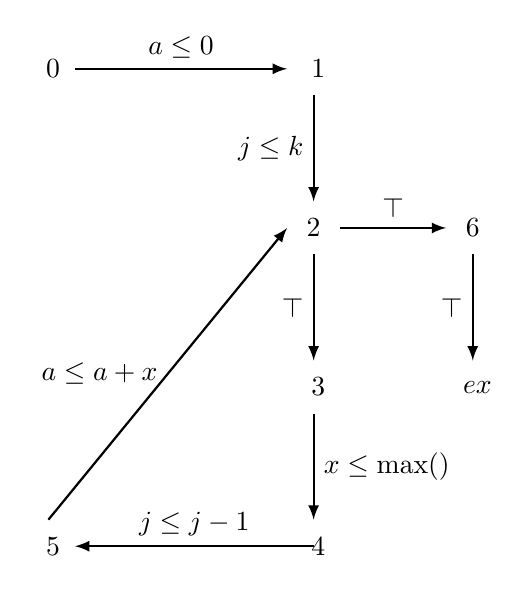
\begin{tikzpicture}[scale=\textwidth/18cm,samples=200]
         \draw[] (-5, 10) circle (0pt) node{{ $0$}};
         \draw[] (0, 10) circle (0pt) node{{ $1$}};
         \draw[] (0, 7) circle (0pt) node{\textbf{$2$}};
         \draw[] (0, 4) circle (0pt) node{{ $3$}};
         \draw[] (0, 1) circle (0pt) node{{ $4$}};
         \draw[] (-5, 1) circle (0pt) node{{ $5$}};
         % Counter Variables
         \draw[] (3, 7) circle (0pt) node {\textbf{$6$}};
         \draw[] (3, 4) circle (0pt) node {{ $ex$}};
         %
         % Control Flow Edges:
         \draw[ thick, -latex] (-4.5, 10)  -- node [above] {$a \leq 0$}(-0.5, 10);
         \draw[ thick, -latex] (0, 9.5)  -- node [left] {$j \leq k$} (0, 7.5) ;
         \draw[ thick, -latex] (0, 6.5)  -- node [left] {$\top$}  (0, 4.5);
         \draw[ thick, -latex] (0, 3.5)  -- node [right] {$x \leq \max(\dbdom)$} (0, 1.5) ;
         \draw[ thick, -latex] (0, 1)  -- node [above] {$j \leq j - 1$} (-4.5, 1) ;
         \draw[ thick, -latex] (-5, 1.5)  -- node [left] {$a \leq a + x$} (-0.5, 7)  ;
         \draw[ thick, -latex] (0.5, 7)  -- node [above] {$\top$}  (2.5, 7);
         \draw[ thick, -latex] (3, 6.5)  -- node [left] {$\top$} (3, 4.5) ;
         \end{tikzpicture}
          \caption{}
            \end{centering}
            \end{subfigure}
            \begin{subfigure}{.33\textwidth}
            \begin{centering}
            \begin{tikzpicture}[scale=\textwidth/18cm,samples=200]
         \draw[] (0, 10) circle (0pt) node
         {{ $a^0: {}^1_{0}$}};
         \draw[] (0, 7) circle (0pt) node
         {\textbf{$x^3: {}^{k}_{1}$}};
         \draw[] (0, 4) circle (0pt) node
         {{ $a^5: {}^{k}_{0}$}};
         \draw[] (0, 1) circle (0pt) node
         {{ $l^6: {}^{1}_{1}$}};
         % Counter Variables
         \draw[] (5, 9) circle (0pt) node {\textbf{$j^2: {}^{1}_{0}$}};
         \draw[] (5, 6) circle (0pt) node {{ $j^4: {}^{k}_{0}$}};
         %
         % Value Dependency Edges:
         \draw[ ultra thick, -latex, densely dotted,] (0, 1.5)  -- (0, 3.5) ;
         \draw[ ultra thick, -latex, densely dotted,] (0, 4.5)  -- (0, 6.5) ;
         \draw[ thick, -latex] (0, 7.5)  -- (0, 9.5) ;
         \draw[ thick, -Straight Barb] (1.5, 3.5) arc (120:-200:1);
         \draw[ thick, -Straight Barb] (6.5, 6.5) arc (150:-150:1);
         \draw[ thick, -latex] (5, 6.5)  -- (5, 8.5) ;
         % Control Dependency
         \draw[ thick,-latex] (1.5, 7)  -- (4, 9) ;
         \draw[ thick,-latex] (1.5, 4)  -- (4, 9) ;
         \draw[ thick,-latex] (1.5, 7)  -- (4, 6) ;
         \draw[ thick,-latex] (1.5, 4)  -- (4, 6) ;
         \end{tikzpicture}
         \caption{}
            \end{centering}
            \end{subfigure}
    \vspace{-0.4cm}
    \caption{(a) The dependency graph for linear regression algorithm 
    (b) The weighted data dependency graph from $\THESYSTEM$}
    \vspace{-0.2cm}
    \label{fig:linear_regression}
\end{figure}
%
Analysis Results: $ \progA(\kw{linearRegression(step, rate)}) = k$
\end{example} 
%
\begin{example}
[Over-approximation Algorithm]
Our algorithm comes across an over-approximation on the estimation due to its path-insensitive nature. It occurs when the control flow can be decided in a particular way in front of conditional branches, while the static analysis fails to witness. 

We use one example to show the over-approximation, Figure~\ref{fig:overappr_example}(a). This example is the variant of the multiple rounds strategy, 
we call it a multiple rounds odd iteration algorithm. In this algorithm, at every iteration, a query $q(b+\chi[i])$ based on previous query results stored in $b$ is asked by the analyst like in the multiple rounds strategy. The difference is that only the query answers from odd iterations ($i =1,3, 5$) are added to $b$. 
  Because the execution trace only updates $b$ using the query answers at odd iterations, so the answers from even iterations do not affect the queries at odd iterations. From the query-based dependency graph in Figure~\ref{fig:overappr_example}(b), we can see that there is no edge from queries at odd iterations (such as $q_1,q_3,q_5$) to queries at even iteration(such as $q_2,q_4$). The longest path is dashed with a length $3$.  However, {\THESYSTEM} fails to realize that odd iteration will always execute then branch and even iteration means else branch, so its dependency graph considers both branches for every iteration. In this sense, the dependency graph by {\THESYSTEM} is similar to the one in the multiple rounds strategy. We show the estimated graph in Figure~\ref{fig:overappr_example}(c). The estimated upper bound is then, $5$, instead of $3$. 
%
\\
Analysis Results: $ \progA(\kw{whileMultiplePath}(k)) = 1 + 2 * k $ --> Over-Approximated
%
{ \small
\begin{figure}
\centering
    \begin{subfigure}{0.3\textwidth}
\centering
\[
    %
    \begin{array}{l}
        \kw{multipleRoundOdd}(k) \triangleq \\
        \clabel{ \assign{j}{k}}^{0} ; \\
        \clabel{ \assign{x}{\query(\chi[0])} }^{1} ; \\
            \ewhile ~ \clabel{j > 0}^{2} ~ \edo ~ \\
            \Big(
             \clabel{\assign{j}{j-1}}^{3} ;\\
             \eif(\clabel{j \% 2 == 0}^{4}, 
             \clabel{\assign{y}{\chi[x]}}^{5}, 
             \clabel{\assign{w}{\chi[x]}}^{6});\\                            
             \clabel{\assign{x}{\query(\chi(\ln(y)))} }^{7} \Big)
        \end{array}
    \]
 \caption{}
    \end{subfigure}
%
\begin{subfigure}{.3\textwidth}
    \begin{centering}
 %   \todo{abstract-cfg for two round}
 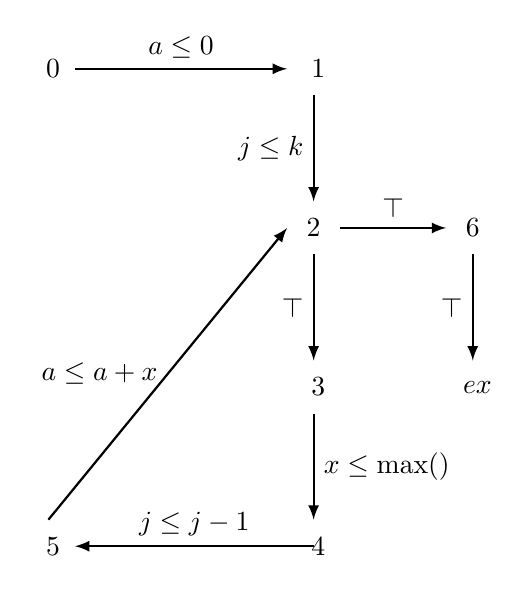
\begin{tikzpicture}[scale=\textwidth/18cm,samples=200]
 \draw[] (-5, 10) circle (0pt) node{{ $0$}};
 \draw[] (0, 10) circle (0pt) node{{ $1$}};
 \draw[] (0, 7) circle (0pt) node{\textbf{$2$}};
 \draw[] (0, 4) circle (0pt) node{{ $3$}};
 \draw[] (0, 1) circle (0pt) node{{ $4$}};
 \draw[] (-5, 1) circle (0pt) node{{ $5$}};
 % Counter Variables
 \draw[] (3, 7) circle (0pt) node {\textbf{$6$}};
 \draw[] (3, 4) circle (0pt) node {{ $ex$}};
 %
 % Control Flow Edges:
 \draw[ thick, -latex] (-4.5, 10)  -- node [above] {$a \leq 0$}(-0.5, 10);
 \draw[ thick, -latex] (0, 9.5)  -- node [left] {$j \leq k$} (0, 7.5) ;
 \draw[ thick, -latex] (0, 6.5)  -- node [left] {$\top$}  (0, 4.5);
 \draw[ thick, -latex] (0, 3.5)  -- node [right] {$x \leq \max(\dbdom)$} (0, 1.5) ;
 \draw[ thick, -latex] (0, 1)  -- node [above] {$j \leq j - 1$} (-4.5, 1) ;
 \draw[ thick, -latex] (-5, 1.5)  -- node [left] {$a \leq a + x$} (-0.5, 7)  ;
 \draw[ thick, -latex] (0.5, 7)  -- node [above] {$\top$}  (2.5, 7);
 \draw[ thick, -latex] (3, 6.5)  -- node [left] {$\top$} (3, 4.5) ;
 \end{tikzpicture}
  \caption{}
    \end{centering}
    \end{subfigure}
    \begin{subfigure}{.33\textwidth}
    \begin{centering}
    \begin{tikzpicture}[scale=\textwidth/18cm,samples=200]
 \draw[] (0, 10) circle (0pt) node
 {{ $a^0: {}^1_{0}$}};
 \draw[] (0, 7) circle (0pt) node
 {\textbf{$x^3: {}^{k}_{1}$}};
 \draw[] (0, 4) circle (0pt) node
 {{ $a^5: {}^{k}_{0}$}};
 \draw[] (0, 1) circle (0pt) node
 {{ $l^6: {}^{1}_{1}$}};
 % Counter Variables
 \draw[] (5, 9) circle (0pt) node {\textbf{$j^2: {}^{1}_{0}$}};
 \draw[] (5, 6) circle (0pt) node {{ $j^4: {}^{k}_{0}$}};
 %
 % Value Dependency Edges:
 \draw[ ultra thick, -latex, densely dotted,] (0, 1.5)  -- (0, 3.5) ;
 \draw[ ultra thick, -latex, densely dotted,] (0, 4.5)  -- (0, 6.5) ;
 \draw[ thick, -latex] (0, 7.5)  -- (0, 9.5) ;
 \draw[ thick, -Straight Barb] (1.5, 3.5) arc (120:-200:1);
 \draw[ thick, -Straight Barb] (6.5, 6.5) arc (150:-150:1);
 \draw[ thick, -latex] (5, 6.5)  -- (5, 8.5) ;
 % Control Dependency
 \draw[ thick,-latex] (1.5, 7)  -- (4, 9) ;
 \draw[ thick,-latex] (1.5, 4)  -- (4, 9) ;
 \draw[ thick,-latex] (1.5, 7)  -- (4, 6) ;
 \draw[ thick,-latex] (1.5, 4)  -- (4, 6) ;
 \end{tikzpicture}
 \caption{}
    \end{centering}
    \end{subfigure}
    \vspace{-0.3cm}
\caption{(a) The labeled program implementing multiple round odd iteration example 
(b) The execution-based dependency graph (c) The program analysis-based weighted dependency graph for the same example.}
    \label{fig:overappr_example}
    \vspace{-0.5cm}
\end{figure}
}
%
\end{example}